\def\layersep{2.5cm}
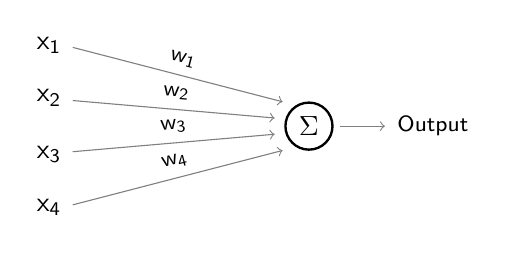
\begin{tikzpicture}[font=\sffamily,shorten >=1pt,->,draw=black!50, node distance=\layersep]
    \tikzstyle{every pin edge}=[<-,shorten <=1pt]
    \tikzstyle{neuron}=[circle,line width=0.3mm,draw=black,minimum size=17pt,inner sep=0pt]
    \tikzstyle{annot} = [text width=4em, text centered]


    \draw[->] (-3,1) -- (-.3,.3) node[sloped,midway,above] {\footnotesize w\textsubscript{1}} node[left=3cm,above=.5cm]{x\textsubscript{1}};

    \draw[->] (-3,0.325) -- (-.4,.1) node[sloped,midway,above] {\footnotesize w\textsubscript{2}} node[left=2.9cm,above=.03cm]{x\textsubscript{2}};
 
    \draw[->] (-3,-.325) -- (-.4,-.1) node[sloped,midway,above] {\footnotesize w\textsubscript{3}} node[left=2.9cm,below=.03cm]{x\textsubscript{3}};
 
    \draw[->] (-3,-1) -- (-.3,-.3) node[sloped,midway,above] {\footnotesize w\textsubscript{4}} node[left=3cm,below=.5cm]{x\textsubscript{4}};
    
    \node[neuron] (0,0) {$\Sigma$};

    \draw[->] (.4,0) -- (1,0) node[right] {\footnotesize Output};
\end{tikzpicture}